% !TEX TS-program = pdflatexmk
% !BIB program = bibtex 

%% -- 
%% -- Chapter A-IV
%% --

%\documentclass[%
%,12pt		% für Korrekturen % wegmachen und Zeilenabstand größer machen
%,oneside]{book}
\documentclass[leqno]{book} 
% Frank N: included [leqno]
%% -- Für das Korrekturlesen
%% --

%\usepackage{setspace}
%\onehalfspacing
%\doublespacing 

%% -- Gemeinsame Pakete und Definitionen
%% --
%% -- Stand 2025/02/14
%% --
%% Welche Pakete verwenden wir 
%% -- 
\usepackage{graphicx}        
\usepackage{libertine}

%% -- Nummerierung Abschnittsweise
%% --
\renewcommand\thesection{\arabic{section}}
\renewcommand\thesubsection{\thesection.\arabic{subsection}}

%% -- AMS-math und mathtools
%% --
\usepackage{amsmath, amssymb, amsthm}	
\usepackage{mathtools}
\usepackage{empheq}
\counterwithin{equation}{section}

%% -- Die Theorem-Umgebungen: Nummerierung nach Abschnitten
%% --

%% --
\theoremstyle{plain}
\newtheorem{theorem}{Theorem}[section]
\newtheorem{proposition}[theorem]{Proposition}
\newtheorem{corollary}[theorem]{Corollary}
\newtheorem{lemma}[theorem]{Lemma} 
%% --
\theoremstyle{definition}
\newtheorem{example}[theorem]{Example}
\newtheorem{examples}[theorem]{Examples} 
\newtheorem{definition}[theorem]{Definition}
%% --
%\theoremstyle{remark}
\theoremstyle{definition}
\newtheorem{remark}[theorem]{Remark}
\newtheorem{remarks}[theorem]{Remark}



%% -- Unsere Pakete
%% --
\usepackage[english]{babel}					% Trennungen richtig
\usepackage{csquotes}						% \enquote{Text} 
\usepackage[inline,shortlabels]{enumitem}	% \begin{enumerate}[(i)] oder [(a)] 
	\setlist{parsep=0.0em}					% etwas enger		
\usepackage{ragged2e}						% \RaggedRight = Flattersatz
%% --
\usepackage{tikz}
\usepackage{tikz-cd}
\usetikzlibrary{matrix,arrows.meta,calc}
%% --
\usepackage{comment}
\usepackage{xspace}

%% --

\usepackage{hyperref}
\hypersetup{
    colorlinks=true,
    linkcolor=blue,
    citecolor=blue,
    urlcolor=blue,
    linktoc=all
}


  
%% -- Definitionen
%% -- Stand 2025/04/14
%% -- var-Symbole für griechisches Alphabet
%% --  Makro zum Tauschen von Symbolen 
%% --

\newcommand{\swapsymbols}[2]{%
  \let\temporaryhold#1%
  \let#1#2%
  \let#2\temporaryhold%
}

%% --  Griechische Buchstaben tauschen
\swapsymbols{\varepsilon}{\epsilon}
\swapsymbols{\varrho}{\rho}
\swapsymbols{\vartheta}{\theta}
\swapsymbols{\varphi}{\phi}

%% --  Vergleichsoperatoren tauschen
\swapsymbols{\leqslant}{\leq}
\swapsymbols{\geqslant}{\geq}


%% -- Zahlen
\newcommand{\N}{\mathbb{N}}		% Natuerliche Zahlen
\newcommand{\Z}{\mathbb{Z}}		% Ganze Zahlen
\newcommand{\Q}{\mathbb{Q}}		% Rationale Zahlen
\newcommand{\R}{\mathbb{R}}		% Reelle Zahlen
\newcommand{\C}{\mathbb{C}}		% Komplexe Zahlen
\newcommand{\K}{\mathbb{K}}		% Koerperzeichen
\newcommand{\T}{\mathbb{T}}		% Torus

%% -- Operatoren					
\DeclareMathOperator{\Id}{Id}
\DeclareMathOperator{\sign}{sign}				% signum-Operator
\newcommand{\im}{\ensuremath{\mathrm{i}}}		% imaginäre Konstante i
\renewcommand*{\Re}{\mathop{}\!\mathrm{Re}}		% Realteil
\renewcommand*{\Im}{\mathop{}\!\mathrm{Im}}		% Imaginärteil
\newcommand*{\supp}{\mathop{}\!\mathrm{supp}\,}  % Träger

%% -- Differential Allgemeine Abkuerzungen
%% --
\newcommand*{\diff}[1]{\mathop{}\!\mathrm{d}{#1}}	% \diff{s} = ds, 
\newcommand*{\ds}{\mathop{}\!\mathrm{d}{s}}       	% \ds = ds, 
\newcommand*{\dg}{\mathop{}\!\mathrm{d}{g}}       	% \dg = dg, 
\newcommand*{\dt}{\mathop{}\!\mathrm{d}{t}}       	% \dt = dt, 
\newcommand*{\dx}{\mathop{}\!\mathrm{d}{x}}       	% \dx = dx, 
\newcommand*{\dy}{\mathop{}\!\mathrm{d}{y}}       	% \dy = dy, 
\newcommand*{\dr}{\mathop{}\!\mathrm{d}{r}}       	% \dr = dr, 
\newcommand*{\dm}{\mathop{}\!\mathrm{d}{m}}       	% \dm = dm, 
\newcommand*{\du}{\mathop{}\!\mathrm{d}{u}}       	% \du = du, 

%% --
\newcommand{\LE}{\mathcal{L}(E)} 		% 
\renewcommand{\L}[1]{\mathcal{L}(#1)} 	% \L{C(K)} zum Beispiel
\newcommand{\BH}{\mathcal{B}(H)} 		% 
\newcommand{\ZE}{\mathcal{Z}(E)} 	% \ZE  Zentrum von E


\newcommand{\Fix}[1]{\mathop{}\mathrm{Fix}\left(#1\right)}		% \Fix{T} Fixraum
\newcommand{\rank}{\mathop{}\!\mathrm{rank}\,}		% 
\newcommand{\Kern}[1]{\mathop{}\mathrm{Ker}(#1)}


%% -- Enpunkt korrekt (momentan ignorieren)
\newcommand*{\eg}{e.g.,\xspace}
\newcommand*{\ie}{i.e.,\xspace}
\newcommand*{\resp}{resp.\xspace}
\newcommand*{\vs}{vs.\xspace}
\newcommand*{\cf}{cf.\xspace}

%% --
\newcommand{\CA}{$\mathrm{C}^{*}$}	% C*-Algebra
\newcommand{\WA}{$\mathrm{W}^{*}$}	% W*-Algbera

%%
\newcommand*{\TT}{\mathcal{T}}		% C_0-Semigroup
\newcommand*{\RR}{\mathcal{R}}		% Pseudo Resolvente
\newcommand*{\SG}{\mathcal{S}}	    % Semigroup
\newcommand*{\UG}{\mathcal{U}}	    % Implemented Semigroup
\newcommand*{\F}{\mathcal{F}}		% F-product
       
%% -- Angepasstes E/F und 1/3
%% -- 1/3

\newcommand*{\sfrac}[2]{\leavevmode\kern.1em%
       \raise.5ex\hbox{\scriptsize #1}%
       \kern-.1em/\kern-.15em%
       \lower.25ex\hbox{\scriptsize #2}}

\newcommand{\nfrac}[2]{\leavevmode\kern.1em%
       \raise.5ex\hbox{\scriptsize #1}%
       \kern-.1em/\kern-.15em%
       \lower.25ex\hbox{\scriptsize #2}}
       
%% -- E/F im Textmodus, sonst \sfrac{E}{F}
%% -- \trfac{E}{F}
%% -- 
\renewcommand{\tfrac}[2]{\raisebox{0.5ex}{#1}\big/\raisebox{-0.5ex}{#2}}
%%

%% -- Eins einer Algebra oder \1_{A} charakteristische Funktion
%% -- 

\usepackage{bbm}
\newcommand{\1}{\mathbbm{1}}

%%KGK
%\theoremstyle{definition}
%\newtheorem*{corollary*}{Corollary}

%% -- O-Spaces
\newcommand{\HO}{\mathcal{H}(O)} 		%  für Lotz
\newcommand{\WO}{\mathcal{W}(O)} 		%  für Lotz

%% -- Differential Allgemeine Abkuerzungen
%% --

\newcommand*{\ddp}{\mathop{}\!\mathrm{d}{p}}       	% \ddp = dp, 
\newcommand*{\dN}{\mathop{}\!\mathrm{d}{N}}       	% \dN = dN, 
\newcommand*{\ddt}{\mathop{}\!\mathrm\fraq{d}{dt}}   % \ddt = d/dt

\newcommand*{\lnm}{LNM1184: } % \LMN-BookCode








%% -- Index 
%% --

%% -- Index 
%% --
\usepackage{imakeidx}
\makeindex[columns=2, options=-s svind.ist]

%% -- Literatur 
%% -- 

\usepackage[round]{natbib}
%Frank N: I use [round], in Ulrich's Version ist is [square, numbers]. I have no idea why.
\bibliographystyle{abbrvnat}

%% --
% Frank N: I included the following definitions:
%\newtheorem*{remark*}{Remark}
%\newtheorem*{remarks*}{Remarks}
\newcommand{\image}{\mathop{}\!\mathrm{im}\,}	

\usepackage{hyperref}
\hypersetup{% 
,colorlinks=true 
,linkcolor=blue
,citecolor=blue
,urlcolor=blue
,linktoc=all
%,hidelinks=true
}

%% -- label prüfen
%%\usepackage{showkeys}  
%% --
           
\begin{document}

%% -- Bitte setzen
%% --

\setcounter{chapter}{3}		%% anpassen 1/2/3 -> Chapter 2/3/4
\setcounter{section}{1}		%% immer

%% -- Das LaTeX-File
%% --

% !TEX root = ../LN-Book.tex
%% --
%% -- Finale Version 2025-06-02
%% -- 
%% --
\chapternopage{Asymptotics of Semigroups on Banach Spaces}\label{chap:a4}%
%\index{Semigroups!Asymptotics}%
%\index{Banach Spaces!Semigroups}
%% --
{\Large
\vspace*{-.75cm}
by \\[.25em]
Frank Neubrander
\vspace{.75cm}
\\
}
%% --
In this chapter, we study the asymptotic behavior of the solutions of the inhomogeneous initial value problem
%% --
\begin{equation}\label{eq:c4-1}
\dot{u}(t) = Au(t) + F(t) \ \text{ for } \  t \geq 0 \ \text{ and } \  
 u(0) = f, \tag{*}
\end{equation}
%% --
where $ A $ is the generator of a strongly continuous semigroup $ (T(t))_{t \geq 0} $ on a Banach space $ E $, and $ F(\cdot) $ is a function from $ \R_{+} $ into $ E $.

In Section 1, we investigate whether -- and at what rate -- a solution $ T(\cdot)f $ of the homogeneous problem converges to the zero solution as $ t \to \infty $. 
In Section 2, we consider the long-term behavior of the solutions of \eqref{eq:c4-1} for different classes of forcing terms $ F $.
%% --
\section{Stability: Homogeneous Case}\label{sec:c4-1}%
%\index{Stability!Homogeneous Case}
%% -- 
Let $ (T(t))_{t \geq 0} $ be a semigroup on $ E $ with generator $ A $.
An initial value $ f \in D(A) $ is said to be \emph{stable} if the solution $ t \mapsto T(t)f $ of
%% --
\begin{equation}\label{eq:c4-2}
\dot{u}(t) = Au(t), \quad u(0) = f \tag{ACP}
\end{equation}
%% --
converges to zero as $ t \to \infty $. 
The semigroup is called stable if every solution converges to zero, \ie if every initial value $ f \in D(A) $ is stable.

If the space $ E $ is finite-dimensional, then the stability of the semigroup implies exponential decay. 
More precisely, the following statements are equivalent.
%%\goodbreak
%% --
\begin{enumerate}[\upshape (a)]
\item 
$ \|T(t)f\| \to 0 $ for every $ f \in \C^{n} $\,,

\item 
$ \|T(t)\| \leq M \mathrm{e}^{-\omega t} $ for some $M \geq 1$ and  $\omega > 0 $\,.
\end{enumerate}
%% --
Moreover, these statements hold if and only if
%% --
%\[
\begin{enumerate}[\upshape (a), resume]
\item 
$s(A) = \sup\{\Re\,\lambda \colon \lambda \in \sigma(A)\} < 0$, 
\end{enumerate}
%\]
%% --
see A-III, Corollary~1.2.

As discussed in Chapter A-III, the situation becomes significantly more intricate in the infinite-dimensional setting. 
For unbounded generators, we must distinguish between \emph{strong} and \emph{generalized (mild)} solutions of $\dot{u}(t) = Au(t)$, as well as between various notions of stability.
If $A$ is the generator of a strongly continuous semigroup on a Banach space $E$ and $f \in D(A)$, then $T(\cdot)f$ is the unique solution or, equivalently, the strong solution of (ACP) with initial value $f$; see A-II, Corollary 1.2 
%\ref{cor:a2-1.2}. 
For an arbitrary $f \in E$, the function $T(\cdot)f$ is referred to as a generalized or mild solution of (ACP). 
Next, we introduce several constants that characterize the growth of solutions of (ACP).
%% --
\begin{definition}($1^{st}$ part)\label{def:a4-1.1} 
Let $A$ be the generator of a strongly continuous semigroup $ (T(t))_{t \geq 0} $ on a Banach space $E$. 
Then we define the following constants.
%% --
\begin{enumerate}[\upshape (i)]
\item 
$\omega(f) \coloneqq \inf\{\omega \colon \|T(t)f\| \leq M\mathrm{e}^{\omega t} \text{ for some } M \text{ and every } t \geq 0\}$ is called the \emph{exponential growth bound} of $T(\cdot)f$,

\item 
$\omega_{1}(A) \coloneqq \sup\{\omega(f) \colon f \in D(A)\}$ is called the \emph{exponential growth bound for the solutions of the Cauchy problem} $\dot{u}(t) = Au(t)$,

\item 
$\omega_{0}(A) \coloneqq \sup\{\omega(f) \colon f \in E\}$ is called the (exponential) \emph{growth bound for the mild solutions of the Cauchy problem} $\dot{u}(t) = Au(t)$.

\end{enumerate}
\end{definition}
%% --
Note that, by the Principle of Uniform Boundedness, 
%% -- 
\[
\sup\{\omega(f) \colon f \in E\} 
= \inf \{ \omega \colon \|T(t)\| \leq M\mathrm{e}^{\omega t} 
    \text{ for some $M$ and every $t \geq 0 $}\}.
\]
%% --
Hence, $\omega_{0}(A)$ coincides with the growth bound of the semigroup $(T(t))_{t \geq 0}$, as defined in A-I, I.3. 
Using the constants defined above, we obtain the following stability concepts.
%% -- 
\setcounter{theorem}{0}
\begin{definition}($2^{nd}$ part)
The semigroup is called
%% --
\begin{enumerate}[\upshape (i), resume]
\item
\emph{uniformly exponentially stable} if $\omega_{0}(A) < 0$,
\item 
\emph{exponentially stable} if $\omega_{1}(A) < 0$,
\item 
\emph{uniformly stable} if $\|T(t)f\| \to 0$ as $t \to \infty$ for every $f \in E$,
\item 
\emph{stable} if $\|T(t)f\| \to 0$ as $t \to \infty$ for every $f \in D(A)$.
\end{enumerate}
\end{definition}
%% --
The interrelation between these stability concepts is given by
%% --
\begin{center}
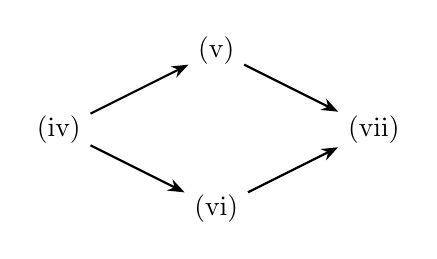
\begin{tikzpicture}[
  node distance=2cm,
  myarrow/.style={-{Stealth[length=6pt]}, thick}
]
% Knoten
\node (iv) at (0,0) {(iv)};
\node (v) at (2,1) {(v)};
\node (vi) at (2,-1) {(vi)};
\node (vii) at (4,0) {(vii)};
% Pfeile
\draw[myarrow] (iv) -- (v);
\draw[myarrow] (iv) -- (vi);
\draw[myarrow] (v) -- (vii);
\draw[myarrow] (vi) -- (vii);
%%
\end{tikzpicture}
\end{center}
%% --
%\[
%\text{(iv)} \Rightarrow \text{(v)} \Rightarrow %\text{(vii)} \text{ and } \text{(iv)} \Rightarrow %\text{(vi)} \Rightarrow \text{(vii)}\,.
%\]
%% --
If $A$ is a bounded operator, that is, if $D(A) = E$, then
%% --
\[
\text{(iv) $\Leftrightarrow$ (v) and (vi) $\Leftrightarrow$ (vii).}
\]
However, if $A$ is unbounded, all stability notions may differ, as illustrated in the following examples.
%%--
\begin{example}\label{ex:a4-1.2}
\begin{enumerate}[\upshape (i), wide, labelindent=.5em]

\item 
Let $E = c_{0}$. 
Then 
%% --
\[
A \colon (x_{n})_{n \in \N} \mapsto (-1/n \cdot x_{n})_{n \in \N}
\] 
%% --
generates the semigroup 
%% --
\[
T(t)(x_{n})_{n \in \N} = (\mathrm{e}^{-t/n} x_{n})_{n \in \N}.
\]
%% --
It is easy to see that $\|T(t)\|=1$ and that $\|T(t)f\|\to 0$ for every $f \in c_{0}$.

Moreover, since $A$ is a bounded operator, $D(A) = E$.
This provides an example of a (uniformly) stable but not exponentially stable semigroup.

The translation semigroups generated by the first derivative on $C_0(\R_{+})$ or $L^{p}(\R_{+})$ for $1 < p < \infty$ offer further examples of (uniformly) stable but not exponentially stable semigroups.

Moreover, as shown in A-II, Example~1.14, the Laplacian $\Delta$ on $C_0(\R^{n})$ generates a bounded holomorphic semigroup given by
%% --
\[
T(t)f(x) = (4\pi t)^{-n/2} \int_{\R^{n}} \mathrm{e}^{-|x-y|^{2}/4t} f(y)  \dy\,.
\]
%% --
This semigroup is not exponentially stable because $0 \in \sigma(\Delta)$ ($\textrm{im}(\Delta) \not= C_0(\R^{n})$); see Corollary~\ref{cor:a4-1.5} below. To see that the semigroup is (uniformly) stable, observe that for every fixed $x\in\R^n$, the kernel $k_t(x,y) := (4\pi t)^{-n/2} \mathrm{e}^{-|x-y|^{2}/4t}$ defines a probability density with $\int_{\R^n} k_t(x,y) \dy\, = 1$. Hence, $\|T(t)\| \le 1$; in fact, $\|T(t)\| = 1$ since $k_t$ also forms an approximate identity. Let $f \in C_0(\R^{n})$ and all $\varepsilon > 0$. Then there exists a compactly supported $g \in C_0(\R^{n})$ such that $\|f-g\| \le \varepsilon$. Therefore,
%% --
\[
\|T(t)f\| \le  \|T(t)\|\|f-g\| + \|T(t)g\| \le \varepsilon + (4\pi t)^{-n/2} \int_{\R^{n}} |g(y)|  \dy\, ,
\]
%% --
which implies  $\|T(t)f\| \to 0$ as $t\to\infty$ for all $f \in C_0(\R^{n})$; see also B-III, Example~1.7.
%%--
This shows that the Laplacian on $C_0(\R^{n})$ (and also on $L^{p}(\R^{n})$ for $1 < p < \infty$, see Example~1.15 below) generates a uniformly stable but not exponentially stable semigroup.

\item 
Note that the condition 
%% --
\[
0 \leq \omega_{0}(A) = \inf\{\omega\colon\|T(t)\| \leq M\mathrm{e}^{\omega t} \text{ for all } t \geq 0\}
\]
%% --
does not exclude the possibility that the semigroup is exponentially stable.

To see this, consider $E \coloneqq C_0(\R_{+}) \cap $ $L^{1}(\R_{+},\mathrm{e}^{x}\dx)$. Then, as shown in A-III, Example~1.3, the translation semigroup satisfies $\|T(t)\| = 1$, and hence $\omega_{0}(A) = 0$. 
For every $\lambda \in \C$ with $\Re\,\lambda > -1$ and every $f \in E$, the resolvent of the generator is given as $R(\lambda,A)f = \int_{0}^{\infty} \mathrm{e}^{\lambda t} T(t)f \,\dt$.
From the equation A-I, (3.2), it follows that
%% --
\[
T(t)f = \mathrm{e}^{\lambda t}\left(f - \int_{0}^{t} \mathrm{e}^{-\lambda s} T(s) (\lambda - A)f  \ds\right),
\]
%% --
and from the existence of the limit
%% --
\[
\lim_{t \to \infty} \int_{0}^{t} \mathrm{e}^{-\lambda s} T(s) (\lambda - A)f  \ds,
\] 
%% --
it follows that 
$\|T(t)f\| \leq M\mathrm{e}^{\lambda t}$ for every $f \in D(A)$ and some constant $M$ depending on $f$. This yields $\omega_{1}(A) \le -1 < 0 = \omega_{0}(A)$. 
Thus, we have a semigroup that is exponentially stable, but not uniformly exponentially stable.

\item
Rescaling this semigroup (see A-I, 3.1), we obtain a semigroup with $\omega_{1}(A) = -1/2 $ and 
$\omega_{0}(A) = 1/2 $.
Therefore, there exist exponentially stable (and hence, stable) semigroups that are not bounded, and hence, not uniformly stable.
This example illustrates that there may be a significant difference between the long-term behavior of the semigroup $(T(t))_{t \geq 0}$ (\ie the set of all mild solutions) and the long-term behavior of the strong solutions $\{T(\cdot)f \colon f \in D(A)\}$ of (ACP). 
\end{enumerate}
\end{example}
%% -- 
In what follows, we characterize the exponential growth bounds $\omega(f)$, $\omega_{1}(A)$, and $\omega_{0}(A)$ in terms of certain abscissas of simple or absolute convergence of the Laplace transform of $T(\cdot)f$. 
These characterizations will serve as one of the tools for 
establishing that, for certain semigroups beyond the class of eventually norm-continuous semigroups (see A-III, Theorem 6.6), the growth bounds $\omega_{0}(A)$ and/or $\omega_{1}(A)$ coincide with the spectral bound $s(A) = \sup\{\Re\,\lambda\colon\lambda \in \sigma(A)\}$. For results of this type, see, for example, B-IV, C-IV, and D-IV.

We begin by observing that $s(A)$ can be interpreted as the abscissa of holomorphy of the Laplace transform $\lambda \mapsto \int_{0}^{\infty} \mathrm{e}^{-\lambda t} T(t) \,\dt$ of the semigroup $(T(t))_{t \geq 0}$.

Furthermore, we recall that the Laplace transform exists for every $\lambda \in \C$ with $\Re\,\lambda > \Re\,\mu$, provided it exists for some $\mu\in\C$.
This follows from 
%% --
\begin{align}\label{eq:a4-1.1}
\int_0^t \mathrm{e}^{-\lambda s} f(s) \ds &= \mathrm{e}^{-(\lambda-\mu)t} \int_{0}^{t} \mathrm{e}^{\mu s} f(s)  \ds \\ 
&+ (\lambda - \mu) \int_{0}^{t} \mathrm{e}^{-(\lambda-\mu)s} \int_{0}^{s} \mathrm{e}^{\mu r} f(r) \,\diff{r} \ds \,. \notag
\end{align}
%% --
Note that even boundedness of 
\[
\left\{ \int_{0}^{t} \mathrm{e}^{-\mu s}f(s)  \ds \colon t > 0\right\}
\]
%% --
implies the existence of the Laplace transform for $\Re\,\lambda > \Re\,\mu$. 
Therefore, the subset of $\C$ for which the Laplace transform exists is always a half-plane 
$\{\lambda \in \C\colon\Re\,\lambda > \gamma\} \cup H$, where $H$ is a subset of the line $\{\lambda \in \C\colon\Re\,\lambda = \gamma\}$.

In the following theorem, we show that the bound of the half-plane for which the Laplace transform of $T(\cdot)f$ ($f \in E$) exists absolutely, and the bound of the half-plane for which the Laplace transform of $T(\cdot)Af$ ($f \in D(A)$) exists strongly, coincide with the growth bound $\omega(f) = \inf\{\omega\colon\|T(t)f\| \leq M\mathrm{e}^{\omega t} \text{ for all } t \geq 0\}$.
%%%%%
%% --
\begin{theorem}\label{thm:a4-1.3}
Let $A$ be the generator of a strongly continuous semigroup $ (T(t))_{t \geq 0} $ on a Banach space $E$. 
Then, for every $f \in E$,
%% --
\begin{equation}\label{eq:a4-1.2}
\omega(f) = \limsup_{t \to \infty} \frac{1}{t}\log\|T(t)f\|, 
\end{equation}
%% --
and
%% --
\begin{enumerate}[(i)]
\item 
$\,\omega(f) = \inf\{\Re\,\lambda\colon\int_{0}^{\infty} \|\mathrm{e}^{-\lambda t} T(t)f\| \,\dt \text{ exists}\}.$
\end{enumerate}
%% --
If\/ $\ker(A) = \{0\}$, then for every $f \in D(A)$ we have
%% --
\begin{enumerate}[(i), resume]
\item 
$\,\omega(f) = \inf\{\Re\lambda\colon\int_{0}^{\infty} \mathrm{e}^{-\lambda t} T(t)Af \,\dt$
\text{ exists}\}.
\end{enumerate}
%% --
\end{theorem}
%%--
\begin{proof}  The proof of \eqref{eq:a4-1.2} is omitted (see \citet[p.306]{hillephillips:1957}. 
To prove (i) and (ii), we need the following lemma.
%% --
\begin{lemma*}\label{lem:a4-1.3}
Let $F \in C(\R_{+},\R_{+})$ be such that $\int_{0}^{\infty} F(r) \dr$ exists. 
If there exist positive constants $m$ and $n$ such that $F$ satisfies the local growth condition $F(t + s) \leq m \cdot F(s)$ for all $s \geq 0$ and $t \in \left[0,n\right]$, then $\lim_{s \to \infty} F(s) = 0$.
\end{lemma*}
%% --
\begin{proof}[Proof of Lemma]
Let $\epsilon > 0$. Since $\int_0^\infty F(r) \dr < \infty$, there exists $a > 0$ such that
\[
A(a) \coloneqq \int_{a}^{\infty} F(r) \dr < \frac{n}{m}\epsilon.
\]
Now fix any $s > a + n$. We claim that there exists $r \in [s - n, s]$ such that
\(
F(r) \leq \frac{1}{n}A(a).
\)
Indeed, suppose that $F(r) > \frac{1}{n}A(a)$ for all $r \in [s - n, s]$. Then
\[ A(a) = \int_{s-n}^{s}\frac{1}{n}A(a)\dr < \int_{s-n}^{s}F(r)\dr \le \int_a^\infty F(r)\dr = A(a), \]
which is a contradiction.
Hence, such an $r \in [s - n, s]$ must exist.
Finally, if $s>a+n$ and $r\in [s-n,s]$, then $0\le s-r\le n$ and, therefore, $F(s) = F(s-r+r) \leq m \cdot F(r) \leq m \cdot \frac{A(a)}{n} < \epsilon$. 
This shows that $\lim_{s \to \infty} F(s) = 0$.
\end{proof}
%% --
To prove part (i) of Theorem~\ref{thm:a4-1.3}, define $b \coloneqq \inf\{\Re\,\lambda\colon\int_{0}^{\infty} \|^{-\lambda t} T(t)f\| \,\dt \text{ exists}\}$. 
A straightforward application of the lemma shows that $\omega(f) \leq b$.
The definition of $\omega(f)$ yields the reverse inequality.

It remains to prove part (ii) of Theorem \ref{thm:a4-1.3}.
Assume that $\ker(A) = \{0\}$ and let $f \in D(A)$, $\lambda \in \C$ with $\Re\,\lambda > \omega(f)$. 
From the equation
%% --
\[
\int_{0}^{t} \mathrm{e}^{-\lambda s} T(s)Af  \ds = \mathrm{e}^{-\lambda t}T(t)f - f + \lambda \int_{0}^{t} \mathrm{e}^{-\lambda s} T(s)f  \ds
\]
%% --
it follows that $\int_{0}^{\infty} \mathrm{e}^{-\lambda t} T(t)Af \,\dt$ exists. 
Therefore, 
%%--
\[c \coloneqq \inf\{\Re\,\lambda\colon\int_{0}^{\infty} \mathrm{e}^{-\lambda t}T(t)Af \,\dt \text{ exists}\} \leq \omega(f).\]
%%--
Next, we show that $c < 0$ implies $c = \omega(f)$. 
For $c < 0$, it follows from \eqref{eq:c4-1} that $\int_{0}^{\infty} T(s)Af  \ds$ exists. 
Since $\int_{0}^{r} T(s)Af  \ds = T(r)f - f$, we see that $g \coloneqq\lim_{r \to \infty} T(r)f$ exists. 
But for every $t \geq 0$, $T(t)g = g$ which implies that $g \in \ker(A) = \{0\}$ or $g = 0$. 
Hence, $\int_{0}^{\infty} T(s)Af  \ds = -f$.
Now, choosing $r < 0$, $b < r < 0$, and integrating by parts, we obtain
%% --
\begin{align*}
-T(t)f &= \lim_{u \to \infty} \int_{t}^{u} \mathrm{e}^{r s} \mathrm{e}^{-r s} T(s)Af  \ds\\
&= \lim_{u \to \infty} ( \mathrm{e}^{ru}\int_0^u\mathrm{e}^{-rs} T(s)Af  \ds - \mathrm{e}^{rt}\int_0^t\mathrm{e}^{-rs} T(s)Af  \ds\\ 
& \qquad \qquad -r\int_t^u \mathrm{e}^{rs}\int_0^s \mathrm{e}^{-rv} T(v)Af\,\diff{v}  \ds
) \\
&= - \mathrm{e}^{rt}\int_0^t\mathrm{e}^{-rs} T(s)Af  \ds -r\int_t^\infty \mathrm{e}^{rs}\int_0^s \mathrm{e}^{-rv} T(v)Af\,\diff{v}  \ds.
\end{align*}
%% --
From $\left\|\int_{0}^{t} \mathrm{e}^{-r s} T(s)Af  \ds\right\| \leq M$ for some $M$ and every $t \geq 0$ we conclude that $\|T(t)f\| \leq \tilde{M}\mathrm{e}^{rt}$ for all $t \geq 0$ and some constant $\tilde{M}$.
Hence, $\omega(f) \leq r$ for every $c < r < 0$, \ie $\omega(f) \leq c$.

If $c \geq 0$ and $w > c$, then $\left\|\int_{0}^{t} \mathrm{e}^{-w s} T(s)Af \ds\right\| \leq M$ for all $t \geq 0$. 
By 
%% --
\begin{align*}
T(t)f - f &= \int_{0}^{t} \mathrm{e}^{w s} \mathrm{e}^{-w s} T(s)Af  \ds\\
&= \mathrm{e}^{wt}\int_0^t \mathrm{e}^{-ws} T(s)Af \ds - w\int_0^t\mathrm{e}^{ws}\int_0^s \mathrm{e}^{-wr} T(r)Af\, \diff{r} \ds,
\end{align*}
%% --
we obtain $\|T(t)f-f\| \leq M\mathrm{e}^{w t} + M(\mathrm{e}^{w t} - 1)
\le 2M\mathrm{e}^{wt}$. 
Hence, $\omega(f)\le w$ for every $w > c$, that is, $\omega(f) \leq c$.
\end{proof}
%% --
Finally, from \eqref{eq:a4-1.2} and the Uniform Boundedness Principle, it follows that the growth bound 
%
\[
	\omega_{1}(A) = \sup\{\omega(f) \colon f \in D(A)\}
\]
%
satisfies
%% --
\begin{align}
\omega_1(A) &={} \inf \{ \omega \colon \text{for every  $f \in D(A)$  there exists a constant $ M $ such that  }\notag \\
& \phantom{xxxxxxxx} \text{ $\|T(t)f\| \leq M\mathrm{e}^{\omega t}$  for every $t \geq 0$} \} \\
&={}
\limsup_{t \to \infty} \frac{1}{t} \log\|T(t)R(\lambda,A)\| \quad (\lambda \in \rho(A)). 
\notag
\end{align}
The following theorem plays a central role in the stability theory of positive semigroups.
We show that the constant $\omega_{1}(A)$ coincides both with the abscissa of simple convergence of the Laplace transform of the semigroup and with the abscissa of absolute convergence of the Laplace transform of the strong solutions of (ACP).
%% --
\begin{theorem}\label{thm:a4-1.4}%
%\index{Theorem!Growth bound}
Let $A$ be the generator of a strongly continuous semigroup $ (T(t))_{t \geq 0} $ on a Banach space $E$. 
Then
%% --
\begin{align}\label{eq:a4-1.4}
\omega_{1}(A) &= \inf\{\Re\,\lambda \colon {\int_{0}^{\infty} \mathrm{e}^{-\lambda t} T(t)f \,\dt} \text{ exists as an improper Riemann} \\
&\phantom{= \inf\{\Re\,\lambda \colon \int_{0}^{\infty} \mathrm{e}^{-\lambda t} T(t)f} \text{integral for every } f \in E\} \notag \\
&= \inf\{\Re\,\lambda \colon {\int_{0}^{\infty} \|\mathrm{e}^{-\lambda t} T(t)f\| \,\dt} \text{ exists for every } f \in D(A)\}.\notag
\end{align}
\end{theorem}
%--
\begin{remarks*}\label{rem:a4-1.4}%
%\index{Remark!Laplace transform convergence}

\begin{enumerate}[\upshape (i), wide, labelindent=.5em]

\item 
One can show that the abscissas of uniform, strong, and weak convergence of the Laplace transform coincide (see C-III, Theorem~I.2, last part of the proof). 
Therefore, by Theorem \ref{thm:a4-1.4},
%--
\begin{align}\label{eq:a4-1.5}
\omega_1(A) &= \inf \left\{ \Re\,\lambda\colon\text{weak-} \lim_{t \to \infty} {\int_0^t \mathrm{e}^{-\lambda s} T(s)  \ds} \text{ exists} \right\}
\\
    &= \inf \left\{ \Re\,\lambda\colon\text{uniform-} \lim_{t \to \infty} {\int_0^t \mathrm{e}^{-\lambda s} T(s)  \ds} \text{ exists} \right\}.\notag
\end{align}

\item
In Equations \eqref{eq:a4-1.4} and \eqref{eq:a4-1.5}, the term \enquote{$\Re\,\lambda$} may be replaced by \enquote{$\lambda \in \R$} (use \eqref{eq:c4-1}).
\end{enumerate}

\end{remarks*}
%% --
\begin{proof}(Proof of Theorem \ref{thm:a4-1.4}) 
The equality 
 \[ 
 \omega_1(A) = \inf \left\{ \Re\,\lambda\colon\int_0^\infty \|\mathrm{e}^{-\lambda t} T(t) f \| \,\dt \text{ exists for all } f \in D(A) \right\} 
 \] 
 follows from the definition of $\omega_1(A)$ and the lemma in the proof of Theorem \ref{thm:a4-1.3}.
We aim to prove that
\[
\omega_1(A) = \inf \left\{ \Re\,\lambda\colon\int_0^\infty \mathrm{e}^{-\lambda s} T(s) f  \ds \text{ exists for every } f \in E \right\}=: b. 
\]
The identity
$    T(t) f = \mathrm{e}^{\lambda t} \left\{ f - \int_0^t \mathrm{e}^{-\lambda s} T(s) (\lambda - A) f  \ds \right\}
$
yields
\[
\omega_1(A) \leq \inf \left\{ \Re\,\lambda\colon\int_0^\infty \mathrm{e}^{-\lambda t} T(t) f \,\dt \text{ exists for every } f \in \text{im} (\lambda - A) \right\}.
\]
Therefore,
$\omega_1(A) \leq b.$
%--
Take $\lambda \in \C$ with $\Re\,\lambda > \omega_1(A)$. 
Then $\int_0^\infty \mathrm{e}^{-\lambda t} T(t) f \,\dt$ exists for every $f \in D(A)$. 
Define $g := \int_0^\infty \mathrm{e}^{-\lambda t} T(t) f \,\dt$. 
Then $g \in D(A)$ and $\int_0^n \mathrm{e}^{-\lambda t} T(t) f \,\dt = \sum_{k=0}^{n-1} \mathrm{e}^{-\lambda k} T(k) g$. 
Since $\text{Re } \lambda > \omega_1(A)$, the sum converges for every $g \in D(A)$. 
Therefore, the integral converges as $n \to \infty$ for every $f \in E$.
For every $t \in \R_+$, define a bounded operator $T_t$ by $ f \mapsto \int_0^t \mathrm{e}^{-\lambda s} T(s) f  \ds$. 
As seen above, $T_n f$ converges as $n \to \infty$ for every $f \in E$. 
It follows from the Uniform Boundedness Principle that $(T_n)_{n \in \N}$ is uniformly bounded.
%%--
%


For every $t \in \R_+$, there exist $n \in \N$ and $t' \in [0,1)$ such that $T_t = T_{t'} + \mathrm{e}^{-\lambda t'} T(t') T_n$. 
Since the operator families on the right side are uniformly bounded, the same is true for $(T_t f)_{t \geq 0}$. 
Since $(T_t f)_{t \geq 0}$ converges for every $f \in D(A)$, it follows that $(T_t f)_{t \geq 0}$ converges for every $f \in E$. 
Thus, $b \leq \omega_1(A)$.
\end{proof}

%%--
%\medskip
%


The inequality
\[
    \omega_{0}(A) \geq \inf \left\{ \text{Re } \lambda\colon\int_0^\infty \|\mathrm{e}^{-\lambda t} T(t) f \| \,\dt 
    \text{ exists for every } f \in E \right\}
\]
combined with the lemma of Theorem \ref{thm:a4-1.3} implies that the growth bound $\omega_{0}(A)$ coincides with the abscissa of absolute convergence of the Laplace transform of $(T(t))_{t \geq 0}$, \ie
\begin{equation}\label{eq:a4-1.6}
   \omega_{0}(A) = \inf \left\{ \text{Re } \lambda\colon\int_0^\infty \|\mathrm{e}^{-\lambda t} T(t) f \| \,\dt \text{ exists for every } f \in E \right\}.
\end{equation}
%--
%


As seen in A-I, Proposition~1.11, if $\int_0^\infty \mathrm{e}^{-\lambda t} T(t) f \,\dt$ exists for every $f \in E$, then $\lambda \in \rho(A)$ and $R(\lambda, A) f = \int_0^\infty \mathrm{e}^{-\lambda t} T(t) f \,\dt$. 
This and Theorem \ref{thm:a4-1.4} yield the following corollary.
%--
\begin{corollary} \label{cor:a4-1.5} Let $ A $ be the generator of a strongly continuous semigroup $ (T(t))_{t \geq 0} $ on a Banach space $ E $. 
Then  
\[
s(A) \leq \omega_1(A) \leq \omega_{0}(A).
\]
\end{corollary}
%% --
Example~\ref{ex:a4-1.2}(c) shows that uniform exponential stability is not equivalent to $ \sigma(A) \subset \{\lambda \in \C\colon\text{Re } \lambda \leq q < 0 \} $. 
The following example shows that even strong solutions can be unstable when $ s(A) < 0 $. We construct a semigroup where $ s(A) < \omega_1(A) < \omega_{0}(A) $.
%% --
\begin{example}\label{ex:a4-1.6} 
As in A-III, Example~1.4, consider the semigroup $ (T(t))_{t \geq 0} $ on the Hilbert space $ E = \{(x^1, x^2, ...) \colon x^n \in \C^n\colon\sum_{j=1}^{\infty} \|x^j\|^2 < \infty\} $, defined by 
\[{
T(t) := (\mathrm{e}^{2\pi i n t} \exp(t A_n))_{n \in \N}
},\]
where
\[
A_n =
\begin{bmatrix}
0 & 1 & 0 & \dots & 0 \\
& 0 & 1 & \dots & 0 \\
& & \ddots & \ddots & \vdots \\
& & & 0 & 1 \\
0 & & & & 0
\end{bmatrix}_{n \times n}.
\]
This semigroup satisfies $ \|T(t)\| = e^t $ for all $t\ge 0$. Hence, $ \omega_{0}(A) = 1 $, while the generator $ A = (2\pi i n + A_n)_{n \in \N} $ has spectral bound $ s(A) = 0 $. 
We first show that $ \omega_1(A) = \omega_{0}(A) $; this will later be used to construct a semigroup for which $ s(A) < \omega_1(A) < \omega_{0}(A) $. 
Let $ e_n = n^{-1/2} (1, ..., 1) \in \C^n $. 

Then, for fixed $n$, 
%% --  
\begin{align*}
\|\exp(&t A_n) e_n\|^2 = \\
&= \frac{1}{n} \left\| (1 + t + \dots + \frac{t^{n-1}}{(n-1)!}, 1 + t + \dots + \frac{t^{n-2}}{(n-2)!}, \dots, 1+t, 1) \right\|^2 \\
&=
\frac{1}{n} \sum_{r=0}^{n-1} \sum_{j,s=0}^{r} \frac{1}{j!s!} t^{j+s} \, = \,
\frac{1}{n} \sum_{r=0}^{n-1} \left(\sum_{j=0}^{r} \frac{1}{j!} t^j \right)^2 
\, = \, \frac{1}{n} \sum_{r=0}^{n-1} \sum_{j,s=0}^{r} \frac{1}{j!s!} t^{j+s} \\
&= 
\frac{1}{n} \sum_{r=0}^{n-1} \sum_{i=0}^{2r} t^i \sum_{j+s=i} \frac{1}{j!s!} \,
= \, 
\frac{1}{n} \sum_{r=0}^{n-1} \sum_{i=0}^{2r} \frac{(2t)^i}{i!} \,  = \,  \frac{1}{n^2} \sum_{i=0}^{n-1} \frac{(2t)^i}{i!}.
\end{align*}
%% --
 For $ 0 < q < 1 $, define $ x_q \in E $ as  
$
x_q := (q e_1, 2q^2 e_2, ..., n q^n e_n, ...).
$
Then $x_q \in D(A)$ and
%--
\begin{align*}
\|T(t)x_q\|^2 & = \sum_{n=1}^{\infty} q^{2n} \| \exp(t A) e_n \|^2
\geq \sum_{n=1}^{\infty} n^2 q^{2n} \left(\frac{1}{n^2} \sum_{i=0}^{n-1}  \frac{1}{i!} (2t)^i \right)\\
&= \sum_{i=0}^{\infty} \sum_{n=i+1}^{\infty} \left( q^{2n} \frac{1}{i!} (2t)^i \right)
= \sum_{i=0}^{\infty} q^{2i+2} (1 - q^2)^{-1} \frac{1}{i!} (2t)^i \\
&= \frac{q^2}{1 - q^2} \sum_{i=0}^{\infty} \frac{1}{i!} (2t q^2)^i
= \frac{q^2}{1 - q^2} \mathrm{e}^{2t q^2}.
\end{align*}
%% -- \noindent kann man sich ersparen, wenn man nach \end{} keine Leerzeile macht, also
%% -- und kein eingerücktes It
It follows that $\omega(x_q) \geq q^2$. 
Thus,
\[
1 = \sup \{\omega(x_q)\colon0 < q < 1\} \leq \omega_1(A) \leq \omega_{0}(A) = 1.
\]
%% --
Rescaling the semigroup (\ie looking at $\mathrm{e}^{-3/2 \cdot t} T(t)$), we obtain a semigroup generator $A$ on the Hilbert space $E$ with $-3/2 = s(A)$ and $\omega_1(A) = \omega_{0}(A) = -1/2$. 
On the other hand, Example~\ref{ex:a4-1.2}(c) produces a semigroup in a Banach space $F$ with generator $B$ such that $-1 = s(B) = \omega_1(B)$ while $\omega_{0}(B) = 0$. 
Now the operator $C := A \oplus B$ on the Banach space $E \oplus F$ is a semigroup generator for which
\[
s(C) = \max \{s(A), s(B)\} = -1, \quad \omega_1(C) = \max\{\omega_1(A), \omega_1(B)\} = -1/2
\]
\[
\text{and} \quad \omega_{0}(C) = \max\{\omega_{0}(A), \omega_{0}(B)\} = 0.
\]
\end{example}
%% -- 
\begin{remark}\label{rem:a4-1.7}
For eventually norm continuous semigroups---particularly compact, differentiable, holomorphic, or nilpotent ones--- the spectral mapping theorem 
%% --
\begin{equation}\label{eq:a4-1.7}
\sigma(T(t)) \setminus \{0\} = \mathrm{e}^{t \sigma(A)}
\end{equation}
%% --
holds. 
Consequently,
%% --
\begin{equation}\label{eq:a4-1.8}
s(A) = \omega_1(A) = \omega_{0}(A)
\end{equation}
%% --
is valid (Corollary \ref{cor:a4-1.5} and A-III, Corollary~6.7).
Hence, if $A$ is the generator of an eventually norm-continuous semigroup, the exponential growth bounds of the strong and mild solutions of the abstract Cauchy problem $\dot{u}(t) = A u(t), u(0) = x$ are determined by the spectral bound
$s(A) = \sup\{\Re\,\lambda\colon\lambda \in \sigma(A)\}.$
\end{remark}
%--
\begin{remark} In general, the growth bound $\omega_{0}(A)$ can be obtained using the Hille-Yosida theorem (see A-II, Theorem~1.7) as
\begin{align}\label{eq:a4-1.9}
\omega_{0}(A) = \inf \{ w\colon\|R(\lambda, A)^n\| \leq &M ( \Re\,\lambda - w)^{-n} \text{ for some } M \text{ and}\\
&\text{every } n \in \N \text{ and } \lambda \in \C \text{ with } \text{Re } \lambda > w\}.\notag
\end{align}
%% --
Due to the difficulty of estimating all powers of the resolvent, this characterization is of limited practical use. 
However, if $A$ is the generator of a semigroup on a Hilbert space $H$, then it is shown in A-III, Corollary~7.11 that
%--
\begin{equation}\label{eq:a4-1.10}
 \omega_{0}(A) = \inf \{ w\colon\| R(\lambda, A) \| \leq M_w \quad \text{for } \Re\,\lambda > w \}.
\end{equation}
\end{remark}
%% --
Unfortunately, the identity \eqref{eq:a4-1.10} does not hold on arbitrary Banach spaces. 
However, as we will see in Section 1 of C-IV, the identity 
%--
\begin{equation}\label{eq:a4-1.11}
 s(A)=\omega_1(A) = \inf \{ w\colon\| R(\lambda, A) \| \leq M_w \quad \text{for } \text{Re } \lambda > w \}
\end{equation}
%% --
holds for every positive semigroup on a Banach lattice. 
Consequently, for positive semigroups with $s(A) = \omega_1(A) < \omega_{0}(A)$ (see Example 
\ref{ex:a4-1.2}~(ii)), the identity \eqref{eq:a4-1.10} is not applicable. 
Nevertheless, we can establish the following theorem.
%% --
\begin{theorem}\label{thm:a4-1.9} 
Let $A$ be the generator of a strongly continuous semigroup $(T(t))_{t \geq 0}$ on a Banach space $E$. 
Suppose there exist constants $a \geq 0$ and $q \geq s(A)$, and that there exist $C > 0$ and $n \in \N$ such that 
%% --
\[
    \| R(\lambda, A) \| \leq C | \lambda |^{n-2}
\]
%% --
for all $\lambda \in \C$ with $\Re\,\lambda > q$ and $| \Im \lambda | > a$. 
Then
%% --
\[
    \sup \{ \omega(f),  f \in D(A^n)  \leq q\}.
\]
\end{theorem}
%% -- 
\begin{proof} 
The hypothesis $\| R(\lambda, A) \| \leq C | \lambda |^{n-2}$ is invariant under rescaling. 
That is, the resolvent $R(\lambda, -b+A)$ of the generator $-b+A$ of the rescaled semigroup $\mathrm{e}^{-bt} T(t)$ satisfies
$\| R(\lambda, -b+A) \| \leq \tilde{C} | \lambda |^{n-2}$ for every $\lambda \in \C$ with $\text{Re } \lambda > q-b$ and $| \text{Im } \lambda | > a+2b$, for a suitable constant $\tilde{C}$. 
Therefore, we may assume without loss of generality that $b := \max(\omega_{0}(A), q) < 0$. 
Let $\omega_{0}(A) < p < 0$, and set $p' := \max\{p, q\} < 0$. 
Then, for every $f \in D(A)$ , the inversion formula for the Laplace transform yields 
\begin{equation} \label{eq:a4-1.12}
T(t) f = \frac{1}{2\pi i} \int_{p' - i\infty}^{p' + i\infty} \mathrm{e}^{\lambda t} R(\lambda, A) f \, d\lambda.
\end{equation}

 (For a proof of the vector-valued inversion formula, see \citet[p.66]{widder:1946}; also refer to the notes in this section.)
Using the resolvent equation, we obtain 
%% --
\[ 
R(\lambda, A)^n R(0, A) = \sum_{k=1}^{n} (-1)^{k+1} \lambda^{-k} R(0, A)^{n+1-k} + (-1)^n \lambda^{-n} R(\lambda, A).
\]
%% --
Since 
$ \frac {1}{2\pi i} \int_{p' - i\infty}^{p' + i\infty} \mathrm{e}^{\lambda t} \, \lambda^{-k} \, d\lambda = 0 $ for $ k \geq 1, p' < 0 $ and $ t > 0$, it follows that
 \begin{equation}\label{eq:a4-1.13}
   T(t) R(0, A)^n f = (-1)^n \frac{1}{2\pi i} \int_{p' - i\infty}^{p' + i\infty} \mathrm{e}^{\lambda t} \lambda^{-n} R(\lambda, A) f \, d\lambda
    \end{equation}
    
 for every $f \in E$ and $t > 0$.
    
 If $q < p'$, then by Cauchy's Integral Theorem and the growth bound $\| R(\lambda, A) \| \leq C | \lambda |^{n-2}$, we can shift the path of integration to 
 $\Re \, \lambda = q$, yielding
 %% --
\[
    T(t) R(0, A)^n f = (-1)^n \frac{1}{2\pi i} \int_{q - i\infty}^{q + i\infty} \mathrm{e}^{\lambda t} \lambda^{-n} R(\lambda, A) f \, d\lambda.
\]
%% -- 
Thus, we estimate  
\[
\| T(t) R(0,A)^n f \| \leq c' \mathrm{e}^{q t} \| f \| \int_{-\infty}^{\infty} (q^2 + s^2)^{-1}\ds = M \mathrm{e}^{q t} \| f \|.
\]
%% --
Equivalently,
%% --
\[
\| T(t) f \| \leq M \mathrm{e}^{q t} \| A^n f \| \text{for $f \in D(A^n)$.}
\]
\end{proof}
%% --
In view of the characterizations given in Section~1 of A-II, the semigroups considered in the theorem above are holomorphic if $ n = 1 $. 
In this case, one may apply \eqref{rem:a4-1.7} to obtain the stronger statement \eqref{eq:a4-1.8}.

Rather than imposing conditions on the resolvent of $ A $, we now adopt a different perspective and characterize the property \enquote{$ \omega_{0}(A) < 0 $} directly in terms of the semigroup $ (T(t))_{t \geq 0} $.
%% --
\begin{proposition} \label{prop:a4-1.10} Let $ A $ be the generator of a strongly continuous semigroup $ (T(t))_{t \geq 0} $ on a Banach space $E$. 
Then the following statements are equivalent.
\begin{enumerate}[\upshape (a)]
\item  
$ \omega_{0}(A) < 0 $.
\item  
$ \lim_{t \to \infty} \| T(t) \| = 0 $.
\item  
$ \| T(t') \| < 1 $ for some $ t' > 0 $.
\end{enumerate}
\end{proposition}
%% --
\begin{proof}
The implications $(a)  \Rightarrow  (b)  \Rightarrow  (c) $ are immediate; To prove $(c)  \Rightarrow  (a) $, note that $\omega_{0}(A) = \lim_{t \to \infty} \frac{1}{t} \log \| T(t) \|$ (see A-I,(1.1)). Assume $\|T(t')\| <1$ for some $t'>0$. For $t=nt'+s$ with $s\in [0,t']$, we have $\|T(t)\|\le \|T(t')\|^n\|T(s)\|$, so that
\[
\displaystyle
\frac{\log \|T(t)\|}{t} \leq \frac{n\log \|T(t')\|}{nt'+s} + \frac{\log \|T(s)\|}{nt' + s}.
\]
Since $\|T(s)\|$ is bounded on compact intervals, the second term tends to zero as $n\to\infty$. The first term tends to $\frac{\log \|T(t')\|}{t'} < 0$. Thus, $\omega_0(A) < 0$, which proves  $(c)  \Rightarrow  (a) $.
\end{proof}
%% --
Other less obvious characterizations of the property 
\enquote{$ \omega_{0}(A) < 0 $} are provided in the following theorem. 
The equivalence of (a) and (c) is known as \emph{Datko’s Theorem}.
%% -- 
\begin{theorem} \label{thm:a4-1.11} 
Let $ A $ be the generator of a strongly continuous semigroup $ (T(t))_{t \geq 0} $ on a Banach space $ E $. 
Then the following statements are equivalent.
%% --
\begin{enumerate}[\upshape (a)]
\item
$ \omega_{0}(A) < 0 $.
\item
$ s(A) < 0 $ and there is $ t_0 > 0 $ such that  
$ |\lambda| < 1$ for every $ \lambda \in A\sigma (T(t_0)).$
\item
For some (equivalently, every) $ p \geq 1 $ the integral $ \int_{0}^{\infty} \| T(t) f \|^p\dt $ exists for every $ f \in E $.
\end{enumerate}
\end{theorem}
%% --
\begin{proof} The implication ``(a) $ \Rightarrow $ (b)'' follows from the fact that $ r(T(t)) = \mathrm{e}^{\omega_{0}(A) t} < 1 $ and $ s(A) \leq \omega_{0}(A) < 0 $. For the point and residual spectrum, the spectral mapping theorem is valid (see A-III, Theorem~6.3). Since the approximate point spectrum is closed, the additional assumption in (b)
implies that $ |\lambda| \leq r < 1 $ for all $ \lambda \in A\sigma(T(t_0)) $. 
Consequently, 
%% --
\[
\exp(\omega_{0}(A) \cdot t_0) = r(T(t_0)) \leq \max\{\exp(t_0 \cdot s(A)), r\} < 1,
\]
%% --
which implies $ \omega_{0}(A) < 0 $. 
This proves \textquotedblleft (b) $\Rightarrow$ (a)\textquotedblright. 
For a proof of the equivalence of (a) and (c), we refer to \citet{datko:1972} or \citet[Theorem~4.4.1]{pazy:1983}. 
\end{proof}
%% --
By rescaling a given semigroup $ (T(t))_{t \geq 0} $, one obtains the following corollary from \eqref{eq:a4-1.1} and statement (c) of the preceding theorem.
%% --
\begin{corollary} \label{cor:a4-1.12} 
Let $ (T(t))_{t \geq 0} $ be a strongly continuous semigroup on a Banach space $ E $. Then the set of $ \lambda \in \C$ for which
\[
\int_{0}^{\infty} \|\mathrm{e}^{-\lambda t} T (t) f \| \,\dt 
\]
exists for every $ f \in E $  is an open right half-plane.
\end{corollary}
%% --
In the next theorem, we present two necessary conditions for the stability of the semigroup $ (T(t))_{t \geq 0} $ in terms of its generator $ A $. 

We will see in Chapter C-IV that for positive semigroups a condition similar to statement (ii) below is even sufficient for stability. 

It is important to note  that stable semigroups need not be uniformly bounded (see Example \ref{ex:a4-1.2}(c)) and that the equality $ s(A) = \omega_{0}(A) = 0 $ does not imply boundedness or even stability of the semigroup (see also A-I, Example~1.4.(i)).
%% --
\begin{theorem} \label{thm:a4-1.13} Let $ A $ be the generator of a stable semigroup $ (T(t))_{t \geq 0} $ on a Banach space $ E $. Then the following assertions hold.
%% --
\begin{enumerate}[\upshape (i)]
    \item 
    $ s(A) \leq 0 $ and $ \operatorname{Re} \lambda < 0 $ for every $ \lambda \in P\sigma (A) \cup R\sigma(A) $.
    
    \item 
    $ \lim_{\lambda \downarrow 0} \lambda R(\lambda, A) f $ exists for every $ f \in D(A) $.
\end{enumerate}
\end{theorem}
%% --
\begin{proof} (i) If $ (T(t))_{t \geq 0} $ is stable, then $ \|T(t) f\| \leq M_f $ for every $ f \in D(A) $. Therefore, $ s(A) \leq \omega_1(A) \leq 0 $. 

Assume, by contradiction, that there exists $ \lambda \in P\sigma(A) $ with $ \Re\,\lambda = 0 $. 
Then, by A-III, Corollary~6.4, there exists $ g \neq 0 $ such that $ T(t) g = \mathrm{e}^{\lambda t} g $ for all $ t \geq 0 $. Since $ |\mathrm{e}^{\lambda t}| = 1 $, this contradicts the stability of the semigroup. 

Now assume there exists $ \lambda \in R\sigma(A) = P\sigma(A') $ with $ \Re\,\lambda = 0 $. 
Then there exists $ 0 \neq \phi \in E' $ with $ T(t)^* \phi = \exp(\lambda t) \phi $ for all $ t \geq 0 $. Choose $ f \in D(A) $ such that $ \langle f, \phi \rangle \neq 0 $. 
Then $ |\langle T(t) f, \phi \rangle| = | \langle f, \phi \rangle| > 0 $ for every $ t \geq 0 $, which again contradicts the stability of the semigroup.

(ii) From the stability of the semigroup and the identity   $\int_{0}^{t} T(s) A f  \ds = T(t) f - f$, it follows that  
$\int_{0}^{\infty} T(s) A f  \ds$ exists for every $ f \in D(A) $.  
Since $ \omega_1(A) \leq 0 $, we may apply Theorem~1.4 to write  $ R(\lambda, A) A f = \int_{0}^{\infty} \mathrm{e}^{-\lambda s} T(s) A f  \ds $ for every $ \lambda > 0 $. 
By a classical theorem of Laplace transform theory, (for a proof of the vector-valued version one may follow \citet[p.196]{widder:1971}), we conclude that $\lim_{\lambda \to 0+} R(\lambda,A)Af$ exists
and is equal to $\int_{0}^{\infty} T(s)Af  \ds$. 
The identity $R(\lambda,A)Af = \lambda R(\lambda,A)f - f$
yields the existence of $\lim_{\lambda \to 0+} \lambda R(\lambda,A)f$ for every $f \in D(A)$.
\end{proof}
%%--
Bounded holomorphic semigroups (see A-II, Definition~1.11) satisfy the estimate
$\|AT(t)\| \leq \frac{m}{t}$ \citet[p.33]{goldstein:1985a}, and hence $T(t)f \to 0$ as $t \to \infty$
for every $f \in \Image{A}$. 
If $\Image{A}$ is dense (\ie $0 \not\in R\sigma(A)$), then we obtain
uniform stability and the following corollary.
%% --
\begin{corollary}\label{cor:a4-1.14}
Let $A$ be the generator of a bounded holomorphic
semigroup $(T(t))_{t \geq 0}$ on a Banach space $E$. 
Then the following statements are equivalent.
%% --
\begin{enumerate}[\upshape (a)]
\item 
$0 \not\in P\sigma(A) \cup R\sigma(A)$.

\item 
$(T(t))_{t \geq 0}$ is uniformly stable.

\end{enumerate}
\end{corollary}
%% --
\begin{example}\label{ex:a4-15}
The Laplacian $\Delta$ generates a bounded holomorphic semigroups on $L^{p}(\R^{n})$ for $1 \leq p < \infty$ (see the example proceeding
Corollary~1.13 in Chapter~A-II). 
All solutions of the equation $\Delta f = 0$ are either constant
or unbounded, so $0 \not\in P\sigma(\Delta)$. 
If $1 < p < \infty$, then the adjoint
of the Laplacian on $L^{p}(\R^{n})$ is the Laplacian on $L^{q}(\R^{n})$, where
$\frac{1}{p} + \frac{1}{q} = 1$. 
Therefore, $0 \not\in P\sigma(\Delta) \cup R\sigma(\Delta)$, and by Corollary \ref{cor:a4-1.14},
the Laplacian generates a uniformly stable semigroup on  $L^{p}(\R^{n})$
for $1 < p < \infty$. However, since $\Image{ \Delta} \not= L^{p}(\R^{n})$, Corollary \ref{cor:a4-1.5} implies that the semigroup is not exponentially stable. %\qed
\end{example}
%%--
As seen in Theorem \ref{thm:a4-1.4}, exponential stability can be characterized by the condition that the abscissa of convergence of the Laplace transform of $(T(t))_{t \geq 0}$ is less than zero. 
This should be compared to the following result, which characterizes (uniform) stability in terms of integrability and the kernel of the generator.
%% --
\begin{theorem}\label{thm:a4-1.16}
Let $A$ be the generator of a strongly continuous semigroup $(T(t))_{t \geq 0}$ on a Banach space $E$. 
The following assertions are equivalent.
%% --
\begin{enumerate}[\upshape (a)]
\item 
$(T(t))_{t \geq 0}$ is stable.

\item 
$\ker(A) = \{0\}$ and $\int_{0}^{\infty} T(t)f \,\dt$ exists for all $f \in \Image{A}$.

\end{enumerate}
%% --
Furthermore the following statements are equivalent,
%% --
\begin{enumerate}[(a')]
\item $(T(t))_{t \geq 0}$ is stable and bounded.
\item $(T(t))_{t \geq 0}$ is uniformly stable.
\item $(T(t))_{t \geq 0}$ is bounded and there is a dense subspace $D$ such that $\int_{0}^{\infty} T(t)f \,\dt$ exists for every $f \in D$.
\end{enumerate}
\end{theorem}

\begin{proof}
If $(T(t))_{t \geq 0}$ is stable, then by Theorem \ref{thm:a4-1.13}, $\ker(A) = \{0\}$, and
\[{
\int_{0}^{t} T(s)Af  \ds = T(t)f - f \to -f \ \text{as} \ t \to \infty\,.
}\]
Hence, $(a) \Rightarrow (b)$.

Conversely, suppose $\int_{0}^{t} T(s)Af  \ds$ converges as $t \to \infty$. Then, by
the identity above, the limit $g \coloneqq \lim_{t \to \infty} T(t)f$ exists. 
Since $\ker(A) = \{0\}$, it follows that $g = 0$, so $T(t)f \to 0$. 
Thus, $(b) \Rightarrow (a)$.

The implication $(a') \Rightarrow (b')$ is immediate. 

If $T(t)f \to 0$ for every $f \in E$, then $\|T(t)\| \leq M$, and $0 \not\in R\sigma(A)$ by Theorem \ref{thm:a4-1.13}. 
Therefore,
$D \coloneqq \Image{A}$ is dense in $E$, and for every $f \in D$, the integral $\int_{0}^{\infty} T(t)f \,\dt$ exists. 
This proves $(b') \Rightarrow (c')$. 

It remains to prove $(c') \Rightarrow (a')$.
Define 
%% --
\[
G \coloneqq \{h \in E \colon h = \int_{0}^{\infty} T(t)g \,\dt \ \text{ for some } \ g \in D\}.
\] 
%% --
We claim that $G$ is dense in $E$. 
Indeed, for any $g\in D$ and $s>0$,  $g - T(s)g \in D$.
Define $h_{s} = \frac{1}{s} \int_{0}^{\infty} T(t)(g - T(s)g) \,\dt = \frac{1}{s} \int_{0}^{s} T(t)g \,\dt$. 
Then $h_{s} \in G$,
and $h_{s} \to g$ as $s \to 0$. 
Therefore, $D \subset \overline{G}$ or $\overline{G} = E$ since $D$ is dense in $E$. 
Now, let $h \in G$, so $h=\int_0^\infty T(t)g\dt$ for some $g\in D$.
Then $T(t)h = T(t) \int_{0}^{\infty} T(s)g  \ds = \int_{t}^{\infty} T(s)g  \ds \to 0$ as $t \to \infty$. 
Since $\|T(t)\| \leq M$, it follows that   $T(t)f \to 0$ for every $f \in E$.
\end{proof}

\begin{remark}\label{rem:a4-1.17}
\begin{enumerate}[\upshape (i), wide, labelindent=.5em]
\item 
If $A$ is the generator of a stable semigroup
$(T(t))_{t \geq 0}$ on a Banach space $E$, then by the previous theorem,
\[{
\Image{A} \subset \{f \in E\colon\int_{0}^{\infty} T(t)f \,\dt \text{ exists}\} =: H\,.
}\]
If $g \in H$, then $\int_{0}^{\infty} T(t)g \,\dt \in D(A)$ and $A \int_{0}^{\infty} T(t)g \,\dt = -g$. 
Thus, $g \in \Image{A}$, and  the dense subspace $\Image{A}$ is given
by
\begin{equation}\label{eq:a4-1.14}
\Image{A} = \{f \in E\colon\int_{0}^{\infty} T(t)f \,\dt \text{ exists}\}
\end{equation}
whenever $A$ generates a stable semigroup $(T(t))_{t \geq 0}$.

\item 
If $\omega(f) < 0$ for every $f \in D(A)$, then $(T(t))$ is stable, but
might not be exponentially stable if
$0 = \omega_{1}(A) = \sup\{\omega(f) \colon f \in D(A)\}$. 
In this case, one can show--via a
proof similar to that of Theorem \ref{thm:a4-1.4}--that the spectrum $\sigma(A)$ must be contained
in the open left half-plane, \ie $\Re\,\lambda < 0$ for all $\lambda \in \sigma(A)$.

\item 
If one defines a semigroup $(T(t))_{t \geq 0}$ to be weakly stable if
$\langle T(t)f,\phi \rangle \to 0$ as $t \to \infty$ for all $f \in D(A)$ and $\phi \in E'$ or as
weakly uniformly stable if the above holds  for all $f \in E$
and $\phi \in E'$, then Theorems \ref{thm:a4-1.13} and \ref{thm:a4-1.16} can be reformulated in a weak form (\ie  replacing stable by weakly stable and \emph{lim} by
\emph{weak-lim}). 
The proofs require only obvious modifications.
If A has a compact resolvent, or if A generates a bounded
holomorphic semigroup, then weak stability implies stability. 
In general, this implication fails; \eg the translation semigroup on
$L^{2}(\R)$ is weakly uniformly stable but not stable (see also B-IV, Example~1.2).
\end{enumerate}
\end{remark}
%% --
\section{Stability: Inhomogeneous Case}%
%\index{Stability!Inhomogeneous Case}
%% --
Using the results of the previous section, we now investigate the long-term behavior of solutions to the inhomogeneous initial value
problem
\begin{equation}\label{eq:a4-2.1}
\dot{u}(t) = Au(t) + F(t) \quad , \quad u(0) = f,
\end{equation}
where A generates a strongly continuous semigroup on a
Banach space $ E $ and $F(\cdot)$ is a locally integrable function from $\R_{+}$
into $ E $, referred to as the \emph{forcing term}. 
A function $u(\cdot)$ is called a \emph{(strong) solution} of \eqref{eq:a4-2.1} if $u(\cdot) \colon \R_{+} \to D(A)$, 
$u(\cdot) \in C^{1}(\R_{+},E)$, and \eqref{eq:a4-2.1} holds for all $t \geq 0$.
The assumption that $A$ generates a semigroup $(T(t))_{t \geq 0}$
guarantees the uniqueness of the solution to \eqref{eq:a4-2.1}. 
If $u(\cdot)$ is a solution, then for fixed $t>0$, the function $v(s) := T(t-s)u(s)$, $0 \leq s \leq t$, is
differentiable and $v'(s) = T(t-s)F(s)$. 
Since $F(\cdot)$ is locally integrable, it follows that 
%% --
\[
\int_{0}^{t} T(t-s)F(s)  \ds = v(t) - v(0) = u(t) - T(t)f.
\]
%% --
Thus, the solution $u(t)$ of \eqref{eq:a4-2.1} is given by
%% --
\begin{equation}\label{eq:a4-2.2}
u(t) = T(t)f + \int_{0}^{t} T(t-s)F(s)  \ds\,.
\end{equation}
%% --
%%%


\begin{example*} \label{ex:a4-2.1}
Let $(T(t))_{t \geq 0}$ be a semigroup that is not eventually differentiable. 
Then there
exists $g \in E$ such that $t \mapsto T(t)g$ is not differentiable on $(0,\infty)$.
Consider the initial value problem $\dot{u}(t) = Au(t) + T(t)g$, $u(0) = 0$. This problem has no
(strong) solution $u(\cdot)$, because otherwise we would have 
\begin{align*}
u(t) = \int_{0}^{t} T(t-s)T(s)g  \ds = tT(t)g,
\end{align*}
which would imply that $t\to T(t)g$ is 
differentiable on $\R_{+}$, a contradiction. 
%\qed
\end{example*}
%%%


Whenever the expression \eqref{eq:a4-2.2} is well-defined, we refer to it as a  \emph{generalized} (or
\emph{mild}) solution of \eqref{eq:a4-2.1}. 
If $F(\cdot)$ is continuous and $f \in D(A)$, then
the generalized solution of \eqref{eq:a4-2.1} is a strong solution if and only if the function 
$v(t) := \int_{0}^{t} T(t-s)F(s)  \ds$ is differentiable (see \citet[Chapter~4,2.4]{pazy:1983}. 
There are several sufficient conditions on the generator A,
the forcing term $F(\cdot)$, or the space $E$ under which every mild solution
is a strong solution of \eqref{eq:a4-2.1} (see \citet{travis:1981}
or  \citet[Section~4.2]{pazy:1983}).

%%%
Our aim in this section is to study the asymptotic behavior of the solutions of \eqref{eq:a4-2.1} as $t \to \infty$. 
To that end, we consider absolutely integrable or periodic forcing terms $F(\cdot)$, and assume that the semigroup
is uniformly stable.

Similar results for integrable and convergent forcing terms $F(\cdot)$ can
be obtained under the assumption of uniform stability (see \citet[p.119]{pazy:1983} or \citet{neubrander:1985b}). 
However, if the
semigroup is positive, these results remain valid even under the weaker assumption of stability (see Section C-IV).
Recall from Theorem \ref{thm:a4-1.13}(i) that for stable
semigroups, the range $\Image{A}$ is dense in $E$.

\begin{theorem}\label{thm:a4-2.1}
Let $A$ be the generator of a uniformly stable semigroup
$(T(t))_{t \geq 0}$ on a Banach space $E$. 
If there exists $g \in \Image{A}$ such that
$\int_{0}^{\infty} \|F(s) - g\|  \ds < \infty$, then every generalized solution $u(\cdot)$ of
\eqref{eq:a4-2.1} converges as $t \to \infty$, and $\lim_{t \to \infty} u(t) = -h$, where $h \in D(A)$ satisfies
$Ah = g$.
\end{theorem}

\begin{proof}
If $u(\cdot)$ is a generalized solution of \eqref{eq:a4-2.1}, then by \eqref{eq:a4-2.2}, we have
\[
u(t) = T(t)f + \int_{0}^{t} T(s)g  \ds + \int_{0}^{t} T(t-s)(F(s)-g)  \ds.
\]
By uniform
stability and the identity $\int_0^t T(s)Ah \ds = T(t)h - h$ (see A-I, Proposition 1.6), the first term converges to zero
and the second term converges to $-h$. 
It remains to show that the
third term also converges to zero. 
Let $\epsilon > 0$ and define $G(s) \coloneqq F(s)-g$. 
Then for any $r>0$,
\begin{align*}
\left\|\int_{0}^{t} T(t-s)G(s)  \ds\right\| & 
{\leq \left\|\int_{0}^{r} T(t-r+r-s)G(s)  \ds\right\| + \left\|\int_{r}^{t} T(t-s)G(s)  \ds\right\|}\\
& 
{\leq \left\|T(t-r)\int_{0}^{r} T(r-s)G(s)  \ds\right\| + M \int_{r}^{\infty} \|G(s)\|  \ds\,},
\end{align*}
where $\|T(t)\|\le M$ for all $t\ge 0$. Since the semigroup is uniformly stable, we obtain
$T(t-r)\int_{0}^{r} T(r-s)G(s)  \ds \to 0$ as $t \to \infty$ for every $r \geq 0$.
Therefore, $\|\int_{0}^{t} T(t-s)G(s)  \ds\| \leq \epsilon$ for all sufficiently large $t$.
\end{proof}


In the following theorem, we show that if A generates a
uniformly stable semigroup, the forcing term $F(\cdot)$ is p-periodic
and $\int_{0}^{p} T(p-s)F(s)  \ds \in \Image{(\Id - T(p))}$, then \eqref{eq:a4-2.1}
 admits a unique p-periodic mild solution that is \emph{asymptotically stable}; \ie for every generalized solution $v(\cdot)$ of \eqref{eq:a4-2.1}, 
%% --
\[
\lim_{t \to \infty} \|v(t) - u(t)\| = 0.
\]  
(Notice that, by
Theorem \ref{thm:a4-1.13} and A-III, Lemma 5.3, $\overline{\Image{(\Id - T(p))}} = E$.)
%% --
\begin{lemma}\label{lem:a4-2.2}
Let $A$ be the generator of a strongly continuous semigroup $(T(t))_{t \geq 0}$ on a Banach space $E$, and let $F(\cdot)$ be a $p$-periodic, locally integrable function with $p > 0$. 
Then the following statements are equivalent.
%% --
\begin{enumerate}[\upshape (a)]
\item 
$\dot{u}(t) = Au(t) + F(t)$ admits a (unique) generalized $p$-periodic solution.

\item 
There exists a (unique) $f \in E$ such that $(\Id - T(p))f = \int_{0}^{p} T(p-s)F(s)  \ds$.
\end{enumerate}
\end{lemma}
%% --
\begin{proof}
(a) $\Rightarrow$ (b): 
Let $f \coloneqq u(0)$ be the initial value for which \eqref{eq:a4-2.1} admits a $p$-periodic mild solution. 
Then for every $t\ge 0$,
%% --
\begin{align*}
u(t) &= u(t+p) \\
&= T(t)T(p)f + \int_{0}^{p} T(t+p-s)F(s)  \ds + \int_{p}^{t+p} T(t+p-s)F(s)  \ds \\
&= T(t)\left[T(p)f + \int_{0}^{p} T(p-s)F(s)  \ds\right] + \int_{0}^{t} T(t-s)F(s)  \ds.
\end{align*}
%% --
Since $u(t) = T(t)f+\int_0^t T(t-s)F(s)\ds$, it follows that
\[T(t)f = T(t)\left[T(p)f+\int_0^pT(p-s)F(s)\ds\right].\]
This implies $f = T(p)f + \int_{0}^{p} T(p-s)F(s)  \ds$.
If $u(\cdot)$ is a unique periodic solution with $u(0) = f$, then $f$ is the unique element in $E$ for which this identity holds.

(b) $\Rightarrow$ (a):  
Define $u(\cdot)$ as in \eqref{eq:a4-2.2}. 
Then
%% --
\begin{align*}
u(t+p) = T(t)\left[T(p)f + \int_{0}^{p} T(p-s)F(s)  \ds\right] + \int_{0}^{t} T(t-s)F(s)  \ds = u(t).
\end{align*}
%% --
If $f$ is unique, then, by the above considerations, the solution is also unique.
\end{proof}
%% --
\begin{remark}\label{rem:a4-2.3}
Let $A$ be the generator of a strongly continuous semigroup for which the spectral mapping theorem holds (see A-III, Section~6), and let $F$ be a $p$-periodic forcing term.
If $\frac{2\pi in}{p} \in \rho(A)$ for every $n \in \mathbb{Z}$, then, by Lemma \ref{lem:a4-2.2}, \eqref{eq:a4-2.1}
admits a unique $p$-periodic solution with initial value $(\Id - T(p))^{-1} \left(\int_{0}^{p} T(p-s)F(s)  \ds\right)$.
\end{remark}
%% --
As a consequence of Theorem \ref{thm:a4-1.13}  and A-III, Corollary~6.4,  a uniformly stable semigroup admits at most one $f \in E$ satisfying 
%% --
\[
(\Id-T(p))f = \int_{0}^{p} T(p-s)F(s)  \ds\,.
\]
%% --
This fact, together with Lemma \ref{lem:a4-2.2}, is used to prove the following theorem.
%% --
\begin{theorem}\label{thm:a4-2.4}
Let $A$ be the generator of a uniformly stable semigroup $(T(t))_{t \geq 0}$ and let $F(\cdot)$ be a $p$-periodic, locally integrable function such that 
%% --
\[{
(\Id - T(p))f = \int_{0}^{p} T(p-s)F(s)  \ds \ \text{ for some } \ f \in E\,.
}
\]
%% --
Then the unique $p$-periodic generalized solution
%% --
\[
u(t) = T(t)f + \int_{0}^{t} T(t-s)F(s)  \ds
\]
%% --
is asymptotically stable.
%% --
\end{theorem}
%% --
\begin{example}\label{ex:a4-2.5}
Let $E$ be the Banach space $C_{0}(\R_{+})$ of continuous functions vanishing at infinity.
Define  $A = \frac{d}{dx}$ with domain $D(A) = \{f \in E: f' \in C^{1} \text{ and } f' \in E\}$ is the generator of the uniformly stable translation semigroup $T(t)f(x) \coloneqq f(t+x)$. 
Applying \eqref{eq:a4-1.14}, we obtain $\Image{A} = \{f\colon\int_{0}^{\infty} f(x) \,\dx \text{ exists}\}$ is dense in $C_{0}(\R_{+})$. 
Let $r \in \Image{A}$ and let $F(\cdot)$ be a $p$-periodic, real-valued function.
We apply Theorem \ref{thm:a4-2.4}  to the initial value problem
%% --
\begin{equation}
 \frac{d}{dt} u(t,x) = \frac{d}{dx}u(t,x) + r(x)F(x+t), \quad u(0,\cdot) \in D(A). 
 \tag{*}
\end{equation}
%% --
We rewrite (*) as  
%% --
\begin{equation}
\dot{v}(t) = Av(t) + G(t), \tag{**}
\end{equation}
%% --
where $v(t) = u(t,\cdot)$ and $G\colon\R_{+} \to E$ is defined by $G(t)(x) = r(x)F(x+t)$.
Then $G$ is $p$-periodic with values in $E$ and $h_{0} \coloneqq \int_{0}^{p} T(p-t)G(t) \,\dt$ is the function $x \mapsto \left[\int_{0}^{p} T(p-t)G(t) \,\dt\right](x) = F(x)\int_{x}^{x+p} r(s)  \ds$. 
Now define $f \coloneqq  \sum_{k=0}^{\infty} T(kp)h_{0}$, which corresponds to the function $x \mapsto F(x)\int_{x}^{\infty} r(s)  \ds$. It is then clear that $(\Id - T(p))f = h_{0}$. 
Therefore, (**) admits a unique $p$-periodic generalized solution by Theorem \ref{thm:a4-2.4}), even though $\im \R \subset \sigma(A)$ (cf. Remark~\ref{rem:a4-2.3}).

The unique $p$-periodic generalized solution $u(t,\cdot)$ is given explicitly by 
%% --
\[
u(t,x) = F(x+t)\int_{x+t}^{\infty} r(s) \ds + F(x+t)\int_{x}^{x+t} r(s) \ds = F(x+t)\int_{x}^{\infty} r(s) \ds.
\]
%% --
Finally, for every solution $v(t,\cdot)$ of (*), Theorem \ref{thm:a4-2.4} implies that
%% --
\[
\sup\left\{\left|v(t,x) - F(x+t)\int_{x}^{\infty} r(s)  \ds\right| \colon x \in \R_{+}\right\} \to 0 \quad \text{as} \quad t \to 0.
\]
%% --
\end{example}
%% --
\section*{Notes}
\addcontentsline{toc}{section}{Notes}
%% --
\begin{enumerate}[label=\emph{Section \arabic*:}, wide, itemsep=1ex]

\item 
The exponential growth bounds $\omega(f)$ and $\omega_{0}(A)$ as well as the characterizations \eqref{eq:a4-1.2}, \eqref{eq:a4-1.6} and Theorem \ref{thm:a4-1.3} (i) can be found in \citet{hillephillips:1957}.
Growth bounds similar to $\omega_{1}(A)$ were first considered in \citet{djacenko:1976} and in \citet[Proposition~2]{zabczyk:1979}. 
Example \ref{ex:a4-1.2}(2) is taken from \citet{wolff:1981}; other \emph{counterexamples} can be found in \citet{hillephillips:1957}, \citet{foias:1973}, \citet{triggiani:1975a}, 
\citet{zabczyk:1975} and \citet{greineretal:1981}. 
Statements \eqref{eq:a4-1.2}, \eqref{eq:a4-1.6} and Theorem \ref{thm:a4-1.3} (i) are semigroup versions of results in classical Laplace transform theory, see \citet{hillephillips:1957} and \citet{widder:1946}. 
Theorem \ref{thm:a4-1.3} (ii) is a semigroup version of Theorem 1.2.7 and 1.2.8 in \citet{doetsch:1950}. 
The lemma in the proof of Theorem \ref{thm:a4-1.3} is taken from \citet{milstein:1975}. 
Theorem \ref{thm:a4-1.4} and Corollary \ref{cor:a4-1.5} can be found in \citet{neubrander:1985a}. 
Example \ref{ex:a4-1.6} follows Remark~2 in \citet{zabczyk:1975}. 
Statement \eqref{eq:a4-1.8} is sometimes called the \emph{spectrum determined growth assumption}, see, for example, \citet{triggiani:1975b}. 
Theorem \ref{thm:a4-1.9} is due to \citet{slemrod:1976}. 
The proof presented here is based on the following sharper version of the inversion formula for the Laplace transform, which improves on the one given in \citet[p.349]{hillephillips:1957}. 
Using \citet[p.66]{widder:1946} or \citet[p.212]{doetsch:1950} one can establish the following theorem (see \citet{neubrander:1984b}.

\begin{theorem}\label{thm:a4-2.6}
Let $A$ be the generator of a strongly continuous semigroup $(T(t))_{t \geq 0}$ on a Banach space $E$. 
For every $f \in D(A)$ and $p > \omega_{1}(A)$ we have
%% --
\[
T(t)f = \frac{1}{2\pi i} \int_{p-i\infty}^{p+i\infty} \mathrm{e}^{\mu t}R(\mu,A)f \, d\mu.
\]
%% --
\end{theorem}
 

The equivalence of the statements \eqref{eq:a4-1.12}, \eqref{eq:a4-1.13} and \emph{$\omega_{0}(A) < 0$} were observed by many authors, see for example, \citet[p.178]{balakrishnan:1976}, 
or \citet{benchimol:1978b}. 
Theorem \ref{thm:a4-1.11} is due to \citet{datko:1970};
for a proof see \citet[p.116]{pazy:1983}. 
Theorems \ref{thm:a4-1.13} and \ref{thm:a4-1.16} can be found in \citet{neubrander:1985b} and Corollary \ref{cor:a4-1.14} is due to \citet{komatsu:1969}. 
An example of an unstable semigroup generator $A$ with Re $\mu < 0$ for all $\mu \in \sigma(A)$ is given in \citet{datko:1983}.

\item For a discussion of well-posedness of inhomogeneous Cauchy problems, we refer to \citet[p.83]{goldstein:1985a}, and \citet[p.105]{pazy:1983}. 
Further results on the asymptotic behavior of the solutions of the inhomogeneous problem can be found in \citet{raohengartner:1974}, \citet{zaidman:1979}, \citet{pazy:1983}, and \citet{neubrander:1985b}. 
Results similar to Lemma \ref{lem:a4-2.2} and Theorem \ref{thm:a4-2.4} are due to \citet{pruess:1984}. 
For a discussion of the asymptotic behavior of the solutions of $\dot{u}(t) = A(t)u(t) + F(t)$ see \citet{datko:1972} and \citet[p.172]{pazy:1983}.

\end{enumerate}

%% -- Literatur
%% --
{\RaggedRight
\bibliographystyle{abbrvnat}
\bibliography{bib/ln-references}}

%% -- Literatur
%% --
%\RaggedRight
\bibliography{LN-Einzelbeitraege/bib/ln-references} 

%% -- Index
%% --

\clearpage
\printindex

%% --
\end{document}
